\appendix
\chapter*{Appendices}
\addcontentsline{toc}{chapter}{Appendices}

\vspace{-1cm}
\setlength{\parindent}{0pt}
\vspace{0.3cm}

\phantomsection
\label{appendix-a}
\section*{Appendix A: Datasets for Khmer OCR Task}

This appendix outlines the publicly available datasets used in the development and evaluation of Khmer OCR models. These datasets include both printed and handwritten Khmer text, covering a wide range of fonts, styles, and input sources. While this list does not represent the full corpus used during research, it includes the key sources that contributed significantly to the training, testing, and evaluation phases.

\begin{itemize}
    \item \textbf{Source 1 – Khmer Printed Text Dataset (62k images)}  
    A large-scale printed text dataset used for both training and evaluation.  
    \url{https://huggingface.co/datasets/SoyVitou/62k-images-khmer-printed-dataset}

    \item \textbf{Source 2 – Khmer Handwritten Dataset (4.2k images)}  
    A dataset containing samples of handwritten Khmer characters and words.  
    \url{https://huggingface.co/datasets/SoyVitou/khmer-handwritten-dataset-4.2k}

    \item \textbf{Source 3 – Updated Khmer Gemma OCR Dataset}  
    Contains improved annotations and updated data for use with Gemma-based models.  
    \url{https://huggingface.co/datasets/KiteAether/update_khmer_gemma_ocr}

    \item \textbf{Source 4 – KhmerOCR-Dataset by lkhapple}  
    A dataset focused on printed Khmer OCR, with paired image-text samples.  
    \url{https://huggingface.co/datasets/lkhapple/KhmerOCR-Dataset}

    \item \textbf{Source 5 – Khmer Gemma OCR Training Subset (Up\_Train)}  
    Curated training data tailored for Khmer OCR with Gemma architecture.  
    \url{https://huggingface.co/datasets/KiteAether/up_khmer_gemma_ocr_train}

    \item \textbf{Source 6 – Khmer Font Printed Dataset}  
    A printed Khmer dataset covering various font styles.  
    \url{https://huggingface.co/datasets/SoyVitou/khmer_font_printed_dataset}

    \item \textbf{Source 7 – Khmer Gemma OCR Evaluation Set}  
    A dedicated evaluation set for benchmarking Khmer OCR performance.  
    \url{https://huggingface.co/datasets 
    KiteAether/up_khmer_gemma_ocr_Evalution_set}

    \item \textbf{Source 8 – Seanghay Khmer OCR Training Set}  
    A Khmer Printed Training set for Khmer OCR Task.  
    \url{https://huggingface.co/datasets/seanghay/khmerfonts}
    info-previews

\end{itemize}

\vspace{0.5cm}

\begin{figure}[H]
    \centering
    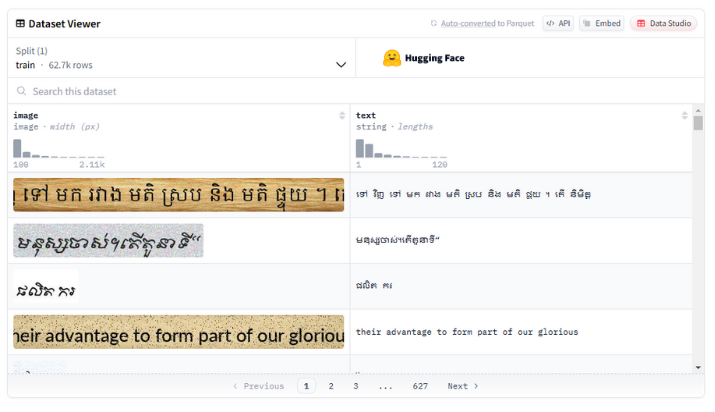
\includegraphics[width=1\textwidth]{figures/khmer_ocr_hugginface_dataset.png}
    \caption{The Khmer-Printed-Text-Dataset (62k images) used for model training and evaluation.}
    \label{fig:khmer_ocr_hugginface_dataset}
\end{figure}

\begin{figure}[H]
    \centering
    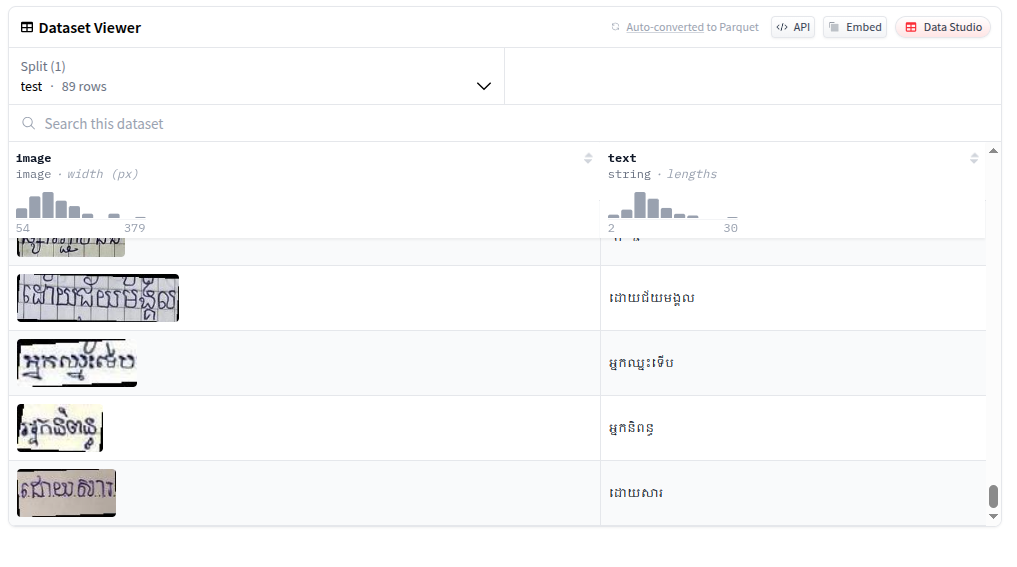
\includegraphics[width=1\textwidth]{figures/khmer_ocr_hugginface_dataset_2.png}
    \caption{The Datasets-KiteAether-up-khmer-gemma-ocr-Evalution-set used for evaluation on Khmer handwritten model, there are 89 images.}
    \label{fig:khmer_ocr_hugginface_dataset_2}
\end{figure}


These datasets enable a variety of OCR research and development tasks, including model training, validation, evaluation, and benchmarking. Researchers and developers can use them to train deep learning models for recognizing Khmer script, conduct font-style generalization studies, assess handwritten text recognition performance, and build production-grade Khmer OCR systems tailored to both digital and scanned documents.


\clearpage
\phantomsection
\label{appendix-b}
\section*{Appendix B: List of Fonts Used}

This appendix lists the Khmer and Latin fonts used during synthetic data generation and model evaluation. Font variability was critical for improving the model's ability to generalize across diverse document styles, layouts, and font renderings. Using a broad range of typefaces helps simulate real-world OCR scenarios, enhancing robustness and accuracy.

\begin{itemize}
    \item \textbf{Source 1 – Google Fonts (Khmer Collection)}  
    A wide variety of Khmer Unicode fonts were collected from Google Fonts.  
    \url{https://fonts.google.com/specimen/Khmer}

    \item \textbf{Source 2 – FontSC Cambodian Fonts Collection}  
    Additional Khmer and Cambodian-style fonts were gathered from this free font archive.  
    \url{https://www.fontsc.com/font/tag/cambodian}
\end{itemize}



\clearpage
\phantomsection
\label{appendix-d}
\section*{Appendix D: Previous Research Using TrOCR}

This appendix highlights prior research efforts related to Khmer handwriting recognition using the TrOCR architecture. The following study represents an important contribution to extending OCR capabilities beyond printed Khmer text.

\vspace{0.3cm}

\textbf{Title:} Khmer Handwritten OCR using Pretrained TrOCR Architecture  
\textbf{Authors:} Soy Vitou, Y Kimly, Lany Malis, Chean Botum  
\textbf{Advisor:} Kor Sokchea  
\textbf{Affiliation:} Department of Information Technology Engineering, Faculty of Engineering, Royal University of Phnom Penh  
\textbf{Project Year:} Year 3

\vspace{0.3cm}

\textbf{Abstract:}  
Most existing OCR models for the Khmer language focus solely on printed text, leaving handwritten text recognition largely unexplored. This limitation reduces OCR's usefulness in areas where handwritten forms are common, such as in schools, government offices, and traditional documents—resulting in inefficiencies due to manual data entry.

This research aimed to:
\begin{itemize}
    \item Develop an OCR model for Khmer handwritten text.
    \item Apply machine learning techniques to improve recognition accuracy.
    \item Bridge the gap between printed and handwritten Khmer OCR applications.
\end{itemize}

While OCR technology has seen significant progress for languages like English in both printed and handwritten forms, Khmer OCR remains underdeveloped, especially for handwriting. To address this, the study developed a Khmer handwritten OCR model using the pretrained TrOCR architecture.

A synthetic dataset of 50,000 printed Khmer text samples was generated using data augmentation techniques—such as noise addition, varied backgrounds, and font variations—for pretraining. A smaller, manually collected dataset of handwritten Khmer samples was then used for fine-tuning the model.

The resulting system demonstrated promising results, achieving a Character Error Rate (CER) of 0.17. Although the model showed an ability to recognize Khmer handwritten text, further improvement is possible through additional fine-tuning and expansion of the training data.

\vspace{0.3cm}

\textbf{Reference:}  
Khmer Handwritten OCR using Pretrained TrOCR Architecture.  
Available at: \url{https://www.researchgate.net/publication/385417010_Khmer_Handwritten_OCR_using_Pretrained_TrOCR_Architecture}  
[Accessed: June 19, 2025]